\documentclass[journal, a4paper]{IEEEtran}
\usepackage[utf8]{inputenc}
\usepackage{graphicx}
\graphicspath{{images/}}
\usepackage{url}
\usepackage{amsmath}
\usepackage{float}

\usepackage{mathtools}
\DeclarePairedDelimiter{\ceil}{\lceil}{\rceil}
\begin{document}

% Define document title and author
  \title{Language Recognition: \\A Deep Neural Network Approach}
  \author{André Pedrosa 85098 \\ Duarte Castanho 85133}
  \markboth{Universidade de Aveiro}{}
  \maketitle

% Write abstract her
\begin{abstract}
Serves the present document as report of Project 2 of the  subject Automatic Learning 
  Topics. Throughout this report we will review some papers researched that have a problem 
  similar to ours. This study proposes a Deep Neural Network approach for Language 
  Identification (LID). We will describe the deep neural network architecture and the machine 
  learning algorithms used as well as the results obtained. In the end we will give an opinion 
  about the work, and what went wrong, the strengths and weaknesses.
\end{abstract}

\section{Introduction}
  \IEEEPARstart{T}{he} duty of Language Recognition involves automatically identifying 
the language in which a given speech was spoken or what language is a text written. 
There are multiple cases of use where LR takes place: multilingual language translation 
(Google translator), emergency or consumer call routing and archaeology.

  There are several approaches already to LID, some of them employing Support Vector 
Machine, others with Gaussian Mixture Model (GMM),  and more recently Deep Neural Networks 
(DNN) and Convolutional Neural Network (CNN) rest on LID approaches are becoming more 
popular, and have been announced to offer equal, and in many cases improved performance
compared to other ways.

% Main Part
\section{State of the art review}
  \IEEEPARstart{T}{here} are a lot of different approaches when it comes to Language Identification.
  In the papers and reports that we reviewed, we ascertained that most of them used a from Neural Network to I-Vectors based approach.
  \begin{itemize}
      \item Paper \cite{1} : The approach to Language Recognition and Speech Recognition 
presented in this paper is using DNN. Their initial DNN experiments focused on 
the Language Recognition task where, in contrast to the Speech Recognition task, 
there were a small number of well defined language classes with a significant 
amount of data for each one.

        For these experiments they used a six language sub-set of the NIST 2009 Language 
Recognition Evaluation (LRE09) corpora that included Farsi, Hindi, Korean, 
Mandarin, Russian and Vietnamese. The training partition consists of 20 hours of 
data per language for a total of 120 hours of speech.

        In this report, it was presented two methods for LR and SP, the direct and 
indirect method. In the direct method for LR and SR, a DNN is used to predict the 
language or speaker class for a given frame of speech. The indirect method uses a 
DNN that was trained on a different data set and possibly for a different purpose. Since 
the entire speech waveform is considered to belong to a single class, the frame-level 
DNN posteriors must be combined to make a single decision score. This was accomplished 
by simply averaging the DNN prediction.

        The DNN used was trained using the training partition of the data set and 
consisted of 819 input nodes, 2 hidden layers with 2560 nodes per layer, and 6 output 
nodes (The six languages). All hidden layers used a Sigmoid activation and the DNN 
learning rate was 0.2.
        \item Paper \cite{2}: In this paper it was presented a tool for learning 
language identification from tagged corpora into a Neural Network.

        The main objective was to use a simple Neural Network implementation, making 
it easy to implement a language identifier in any programming language given the 
neural network parameters T, then apply new techniques, namely the referred deep 
neural networks. The Network Architecture is composed by a set of L layers, where 
the first layer has 565 units (total number of characters in all alphabets used) the 
output layer has 25 units (all languages used) where each one gets a value between 0 
and 1 which is the probability of that text being that language.
  After adding the alphabet features, aftewards they trained the neural network with two different
number of iterations: 1500, and 4000. Globally, with 1500 iterations it was possible to get 96\% of
precision, and with 4000 iterations it got up to 97%.

        The training set size used was between 500.000 and 1.087.000 words per language and the test set ranged from 270 to 15.000 words.
        \item Paper \cite{4}: Deep Convolutional Recurrent Neural Networks: 
    This type of NN are a combination of convolutional NN and recurrent NN.

    For a problem like, for example, object recognition where we have big sized images with hundreds 
or thousands of pixies a neural network receive this pixels as input data, and can respond to the 
problem. However, they fail to capture some important details such as the correlation between parts of 
the image. What a convolutional neural network (CNN) does is extract local features merging them to be 
used as higher-order features for more convolutional layers or for other type of neural network as the 
case of the paper in question. Can be called a feature extractor.

    In this paper the problem exposed was to receive a audio sequence and identify the language of the 
sound. Because a sound can have so much data for a simple neural network, the data goes through a 
CNN to extract relevant features.
    We can simply think that in this problem data of a sound file is correlated, so a sound on a 
specific time it only makes sense with their neighbours. FeedForward NN don't handle this very well, 
thus having to introduce more features on the NN. To solve this, the authors mixed a CNN, to capture 
spatial information, to a recurrent neural network (RNN) to capture information through a sequence 
of time steps, forming a deep convolutional recurrent neural network (CRNN).

    A RNN brings better performance as the output of its nodes are directed to two directions. One 
is to one or more nodes of the next layers of the NN and the other is to one or more nodes in the 
same layers, allowing the NN to have a internal state, which allows a great performance on sequence inputs.

      The input data was sound spectrograms that were fed into the CNN. The part of the RNN was 
implemented with a bidirectional long-short term memory (BLSTM) using two (\textit{Long-short 
Term Memory}) (LSTM) networks. Their output was concatenated as this output was feed into 
a fully-connected layer that served as a classifier.

      In what concerns the experiments done by the authors of this paper they had two datasets to train
the NN splitting each one into tree sets, training (70\%), validation (20\%) and test (10\%). The first
dataset had 19000 training images (53 hours of speech audio) and the second with 194000 training images
(540 hours of speech audio). Both datasets had samples from four different languages (English, french,
german and spanish). Their first step was to see the difference of performance between a CNN
and a CRNN with the first dataset. The CRNN architecture outperformed the plain network significantly having
an accuracy of 98\% against an accuracy of 90\% of the CNN. On a second phase they used the other dataset
to train the CNN trained with the previous set and trained four more models from scratch (CNN, CRNN, 
Inception-v3 CNN, Inception-v3 CRNN \cite{inceptionv3}). The model already trained was the one with
worst performance having an accuracy of 79\%. The authors explain that this happen because the first dataset
does not feature such a diverse range of situations, as the second dataset. On this dataset the CNN and
CRNN architectures didn't have that much of a difference with only 1\% of difference between them (
CNN 90\% and CRNN 91\%). The new models using Inception-v3 had a better performance with an increase of
5\% on accuracy (Inception-v3 CNN 95\% and Inception-v3 CRNN 96\%). From this results they extracted that
deeper models tend to capture more general features, however this increase comes with a increase of
computational cost. The authors also tested the robustness of the CRNN and Inception-v3 CRNN models
against noise. They inserted three types of noise, white noise, crackling noise (simulate a bad voice
connection) and with a background music. As expected the noise affected the results but in a more
serious way on the CRNN architecture with a drop of accuracy up to 21\%. The architecture with
Inception-v3 CRNN only had a drop of 7\% on accuracy. The authors say that this happens because
the Inception-v3 CRNN, with its deeper and more complex structure, is able to capture the frequency
features in a more robust manner. On the final experiment they tested how well their CRNN model
would perform with an addiction of two more languages to the second dataset (Russian and mandarin).
The model got an accuracy of 92\% against the 91\% obtained before. This proves that the CRNN architecture
proposed can easily be extended to cover more languages
  \end{itemize}

\section{Data description, visualization and statistical analysis}
    Our LID problem is to predict to which language a given word most likely belongs.

    To build our data sets we used the lists of words of the website \cite{website} of the languages:
    \begin{itemize}
      \item english
      \item french
      \item german
      \item italian
      \item spanish
    \end{itemize}
    In addition we also used a list of portuguese words from \cite{website2}. In total we have 6 
languages, in other words we have 6 classes for our ML algorithms.

    Because different words have different lengths and a machine learning (ML) algorithm have a 
defined length for its input, a preprocessing is required before feeding the words into the ML 
algorithms.

\section{Data Preprocessing}
    From each language we ignored the words that:
    \begin{itemize}
      \item have other characters besides letters, e.g. dots, dashes, \ldots
      \item have less then 4 letters or more than 12 letters
    \end{itemize}
    To each word we also did a transformation converting non-ascii letter to ascii,
e.g. the german letter ü would be transformed into an u.
    As it can exist more words in one language than others, one language can be better classified 
than others, to solve that, we did a selection of words within each language to make all languages 
have the same number of words. Doing this the number of words per language is limited by the 
language that has less amount of words. This number (From now on we will call this value of m) 
in our case was 83077, that is for each language we got 83077 words, what give us a total of 
\(83077*6=498462\) examples/words.

    The next step is to extract m words for each language since they have different total number 
of words, but we can't just take the first m words because they can have the same pattern, e.g. 
all begin with the letter 'a' leading to a bad data set. To solve this we implemented an algorithm 
based on the linspace MATLAB function that give us m indices of words to consider from a language 
starting at 1 and ending at the number of words in that specific language.
    Having this, we split the data from each language into training (60\%), validation(20\%) 
and test data(20\%) using the same algorithm mentioned above and them merge them all into 
three big sets, again training (\(\ceil[\big]{83077*0.6}*6=49846*6=299076\) examples), validation 
(\(\ceil[\big]{83077*0.2}*6=16615*6=99690\) examples) and test data 
(\((83077-49846-16615)*6=16616*6=99696\) examples).

    Now the selected words need some transformation so they can be used by ML algorithms as input 
data because they have different lengths. For that we transformed each word into a binary array, 
where each letter is a binary number. Because there are 26 letters, we need 
\(\ceil[\bid]{\log_2 26}=5\) bits to represent a letter.\\

    a = 00001

    b = 00010

    c = 00011

    ...

    z = 11010\\

    A word is a combination of \(5*12\) (12 is the maximum length for a word) bits. Additionally
padding may be needed for words with less than 12 letters. For that for each missing letter we 
insert 5 zeros. Each bit on these binary arrays will be a feature of our ML models.

\section{Description of the applied machine learning algorithms}
    To solve our problem we developed a deep neural network (DNN). An artificial neural 
network (ANN) consists of input and output layers as well as hidden layers that makes 
transformations on the input into something that makes sense on the output. Each layer 
can have several units. A DNN is an ANN with multiple hidden layers.

    Furthermore, we solved the problem using Support Vector Machine (SVM) to compare 
the results of both algorithms. SVM is a supervised machine learning algorithm that for 
a given example set, marks as belonging to one of two classes. As SVM only work 
for two classes, a classification strategy of \textit{one against one} was used to have 
a multiclass classification.

    For both DNN and SVM we followed the same methodology to find the best model.
    \begin{enumerate}
      \item We determine a range for each hyper parameter and create all possible 
        combinations of them
      \item Each model is trained with the training data (60\%).
      \item We get the score of these models over the validation data (20\%) and choose
        the model with the best score.
      \item This best model is then trained with the training and validation data 
        (80\%) using the model already trained with the training data from the previous 
        stage.
      \item Finally we use the test data to get the final score of our final models.
    \end{enumerate}
    For the DNN we used \textit{Keras: The Python Deep Learning library} with 
TensorFlow backend. This library provides several optimizers for the training of the NN, consequently
we created several models where for each optimizer we tested different NN structures with
different number of units per layer and different number of layers.

    The optimizers are:
    \begin{itemize}
      \item SGD - Stochastic gradient descent
      \item RMSprop
      \item Adagrad
      \item Adadelta - extension of Adagrad \cite{adadelta}
      \item Adam \cite{adam}
      \item Adamax - variant of Adam \cite{adam}
      \item Nadam \cite{nadam}
    \end{itemize}
    The structures are (each number represents the number of units of a hidden layer):
    \begin{itemize}
      \item 200, 150, 100, 100
      \item 200, 100, 50
      \item 200, 100
      \item 100, 50,  25,  25
      \item 100, 50,  25
      \item 100, 50
    \end{itemize}
    Giving a total of 42 models created and tested. Each model was trained using 400 epochs.

    For the SVM we used \textit{scikit-learn} that is another Python module for machine 
learning built on top of SciPy. For SVM classification this library offers several kernel types.
We used:
    \begin{center}
      \begin{tabular}{ |c|c| }
        \hline
        \textbf{Kernel name} & \textbf{Kernel function} \\
        \hline
        Linear & \(X^{T}X'\) \\
        \hline
        Gaussian (RBF) & \( exp(-\gamma.\parallel X-X'\parallel^{2})\) \\
        \hline
        Sigmoid & \(tanh(\gamma.X^{T}X'+coef0)\) \\
        \hline
      \end{tabular}
    \end{center}
    The Gaussian and Sigmoid kernel has a \textit{gamma} (\(\gamma\)) hyper parameter that defines how 
much influence a single training example has. The larger gamma is, the closer other 
examples must be to be affected. This parameter we tested with two values, auto and scale. 
For auto the library sets the gamma parameter to \(1/n\_features\) and for scale sets to
\(1/(n\_features*X.std())\), where X is the matrix of training examples and the function 
\textit{std} returns the standard deviation of the flatten matrix X.

    The Sigmoid kernel has a \textit{coef0} hyper parameter that defines the independent 
term in kernel function. For this parameter we used the value -25, 0 , 25.

    All the kernels have a common hyper parameter that is the parameter \textit{C} that 
trades off misclassification of training examples against simplicity of the decision 
surface. A low C makes the decision surface smooth, while a high C aims at classifying 
all training examples correctly. This parameter we used two different range of values.
In a first phase we used 0.001, 1 and 30. After that we would see what kernel would do better
and also trained more models of that kernel with C being 0.01, 0.1, 10 and 20. Our best model
was the Gaussian kernel so in total we trained 35 models for the SVM ML algorithm (3 with linear
kernel, 18 with kernel Sigmoid (2 values of gamma, 3 values of C and 3 values of coef0), 14 with kernel
Gaussian (2 values of gamma and 7 values of C)).

\section{Presentation and discussion of results}
    \subsection{DNN}
    At first we ran our model with 200 epoch and obtained some models where
  a stabilization wasn't clear (see figure \ref{fig:sgd_200_100}), consequently we 
trained all the model with more 200 epochs with a total of 400.

    \begin{figure}
      \center{
        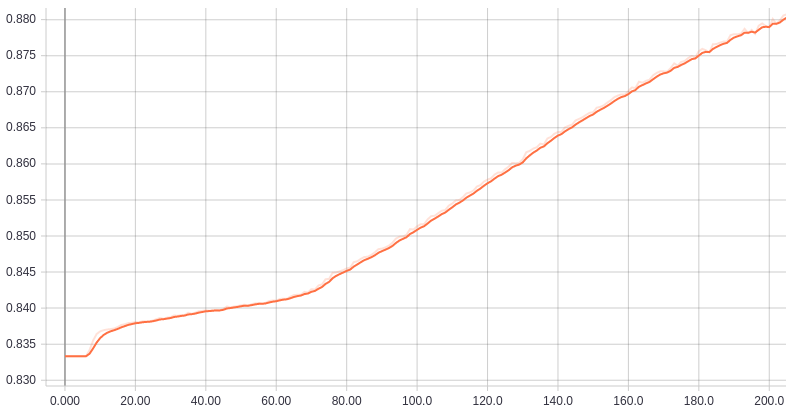
\includegraphics[scale=0.35]{sgd_200_100.png}
      }
      \caption{Validation accuracy of the model with SGD optimer and
      a DNN with two layers with 200 and 100 units each}
      \label{fig:sgd_200_100}
    \end{figure}

    However the majority of the models was already overfiting with 200
epochs. On figure \ref{fig:adam_200_100} we can clearly see this
phenomenon.

    \begin{figure}
      \center{
        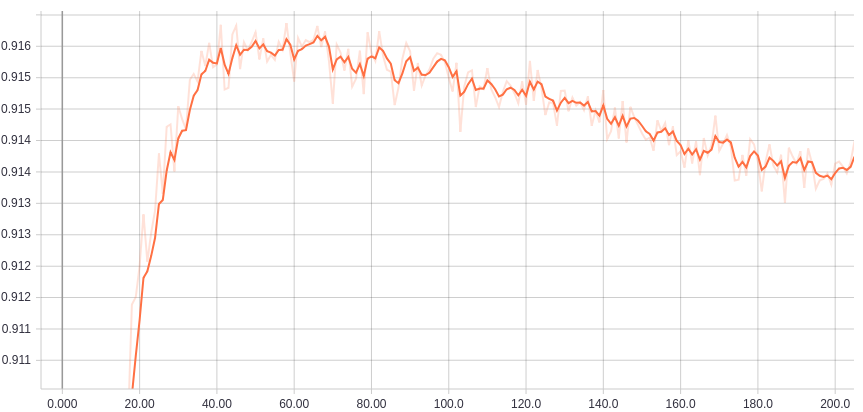
\includegraphics[scale=0.32]{adam_200_100.png}
      }
      \caption{Validation accuracy of the model with Adam optimer and
      a DNN with two layers with 200 and 100 units each}
      \label{fig:adam_200_100}
    \end{figure}

    After running all the 400 epochs for all models our best model
used the Adadelta optimizer with two hidden layers with 200 and 100 units
with a validation accuracy of 91,70\%. On figure \ref{fig:cross_val_dnn}
we can compare the several models among them. \\ We can see clear differences of performances
between some optimizers such as SGD and Adagrad from RMSprop. The Adam based optimizers all
have a good performance average for all structures, having just a difference of around
0,2\% from the best model. \\
    We expected that the structures with more units and more deep layers had
better performance but this results counter our expectations, since that the best model
only has two layers.

    \begin{figure}
      \center{
        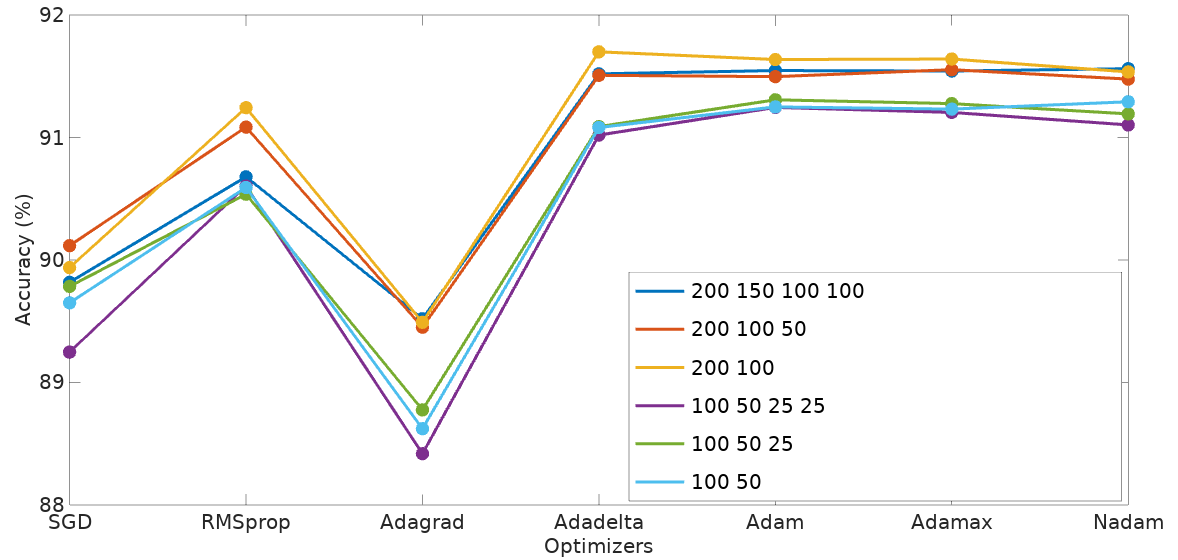
\includegraphics[scale=0.22]{cross_val_dnn.png}
      }
      \caption{Cross-validation accuracy of the DNN models. The lines are just to
      facilitate the comparison between structures using the same optimizer, because
      the x axis is discrete}
      \label{fig:cross_val_dnn}
    \end{figure}

    Afterwards, we retrained the best model with train and validation data and
we obtained more 0.096\% on our model with a total of 91,7968\%. On figure
\ref{fig:dnn_final} we can see the evolution's performance relatively to the
last model, having some traces of overfit.

    \begin{figure}
      \center{
        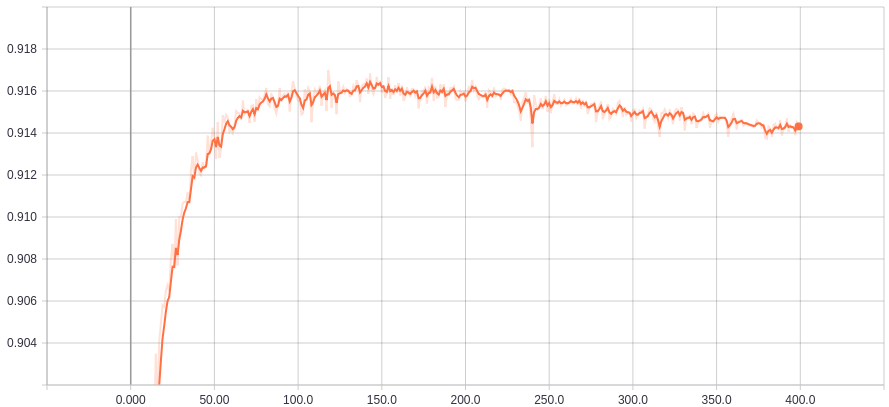
\includegraphics[scale=0.29]{dnn_final.png}
      }
      \caption{Evolution of the accuracy of the last model during training}
      \label{fig:dnn_final}
    \end{figure}

    \subsection{SVM}
    As said on the previous section the SVM models went through two phases. On the first
phase we trained using three values of C (a hyper parameter shared for all models), use gamma
with value 'scale' and 'auto' and the ones that use the coef0 hyper parameter set it to
-25, 0 and 25.

    \begin{figure}
      \center{
        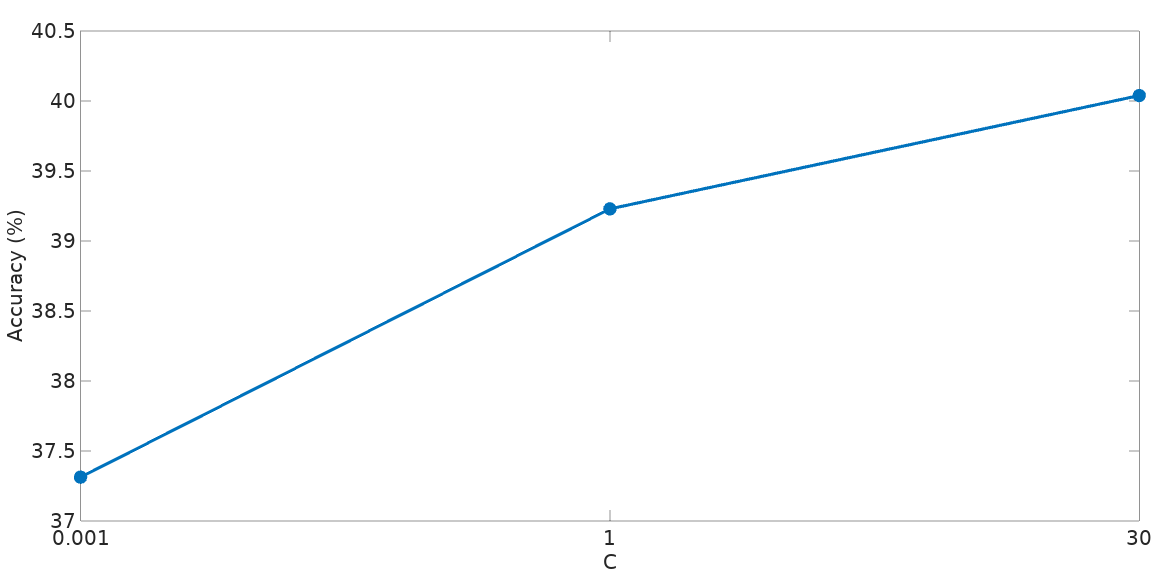
\includegraphics[scale=0.22]{linear.png}
      }
      \caption{Performance of the several models using a linear kernel}
      \label{fig:svm_linear}
    \end{figure}

    The linear model only as the C hyper parameter so we only tested three models, one
for each C. The results are on figure \ref{fig:svm_linear}. We can clearly see that the increase
of C brings more performance to the model but no where near to the accuracy found on the DNN models.

    \begin{figure}
      \center{
        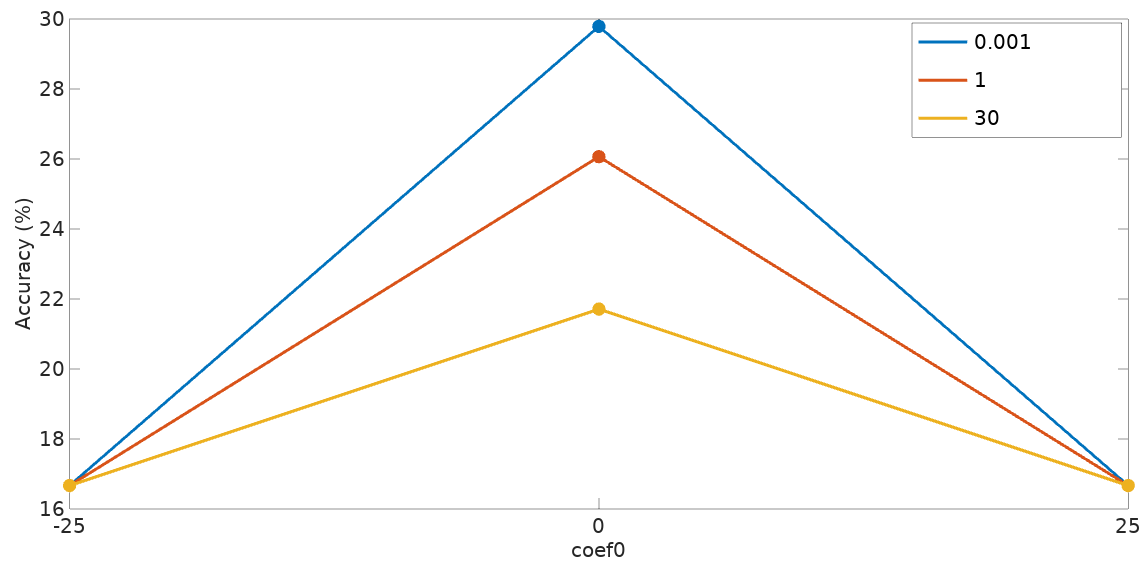
\includegraphics[scale=0.23]{sigmoid_auto.png}
      }
      \caption{Accuracy of the several models using a sigmoid kernel with gammas as auto. On the legend
      are the several values of C used}
      \label{fig:svm_sigmoid_auto}
    \end{figure}

    The sigmoid kernel has C, coef0 and gamma as hyper parameters having the higher number of models
to training. On the figure \ref{fig:svm_sigmoid_auto} we have the accuracy of the models using
gamma as auto. Here the variation of the coef0 brings the performance down as \(coef0=0\) as the best
results. The variation of the C value only has impact when \(coef0=0\) with lower the C the higher
the performance is.

    \begin{figure}
      \center{
        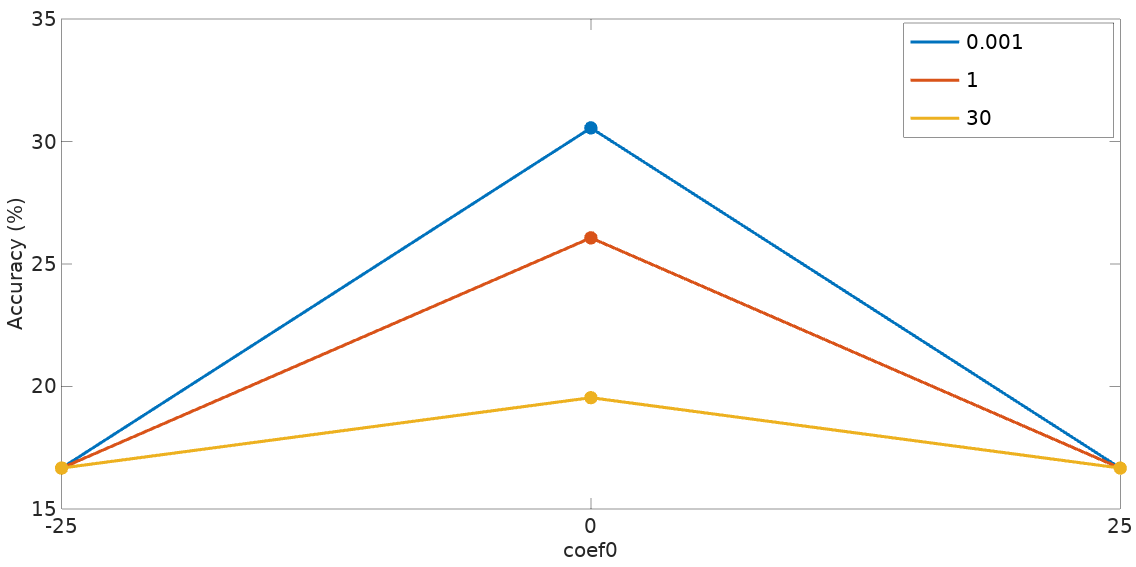
\includegraphics[scale=0.23]{sigmoid_scale.png}
      }
      \caption{Accuracy of the several models using a sigmoid kernel with gammas as scale. On the legend
      are the several values of C used}
      \label{fig:svm_sigmoid_scale}
    \end{figure}

    On figure \ref{fig:svm_sigmoid_scale} we are using gammas as scale with the same sigmoid kernel and we
can see that the results have the same pattern with a lower accuracy value. As linear kernel results, they
don't come near the ones obtained with DNN.

    \begin{figure}
      \center{
        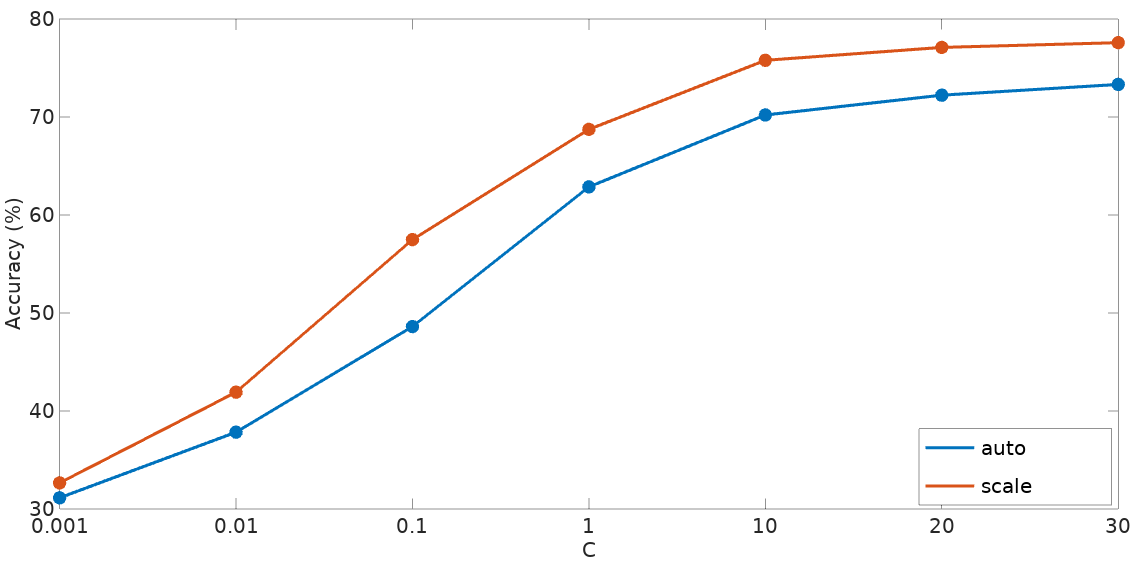
\includegraphics[scale=0.23]{rbf.png}
      }
      \caption{Accuracy of the several models using a Gaussian kernel. On the legend
      are the several values of gamma}
      \label{fig:svm_rbf}
    \end{figure}

    Our best results with SVM was achieved using the Gaussian (RBF) kernel with a \(C=30\) and gamma
set to scale with an accuracy of 77.59\%. So this kernel went to the second phase where we train more 4 models for each gamma
with different values of C (0.01, 0.1, 10 and 20). We end up not finding a better model so we retrained
the best model with the train and validation data and we increased the accuracy to 78.57\%. On the
figure \ref{fig:svm_rbf} we can clearly see the difference between gamma equal to auto and scale. Furthermore, on
Gaussian kernel the C has a significant impact, showing an increase on performance of around 30\% from the
\(C=0.001\) to \(C=30\).

    \subsection{Comparison}
    From the results we cannot say that the DNN has a substantial performance over the SVM, as we can still have a positive
satisfactory/good classification by the SVM model. Although it is clear that the DNN model is better than
the SVM, having around 13\% difference in performance.

    In terms of computing time, our expectations were that the DNN would take a serious amount of time to train
just one model and the SVM would be fast as we could train fewer model from one and a lot from the other.
End up being the other way around. We trained all our DNN models with 400 epochs in approximately 2 days
on only one computer, but the SVM we had to split our multiple models and run them on more than one computer
at the time taking us more than 4 full days to train all models. This can be a consequence of how well
the libraries used have implemented the parallelization of the of training. During the training of the DNN
the training of one model we could see that was using all the 4 cores while the SVM training was only taking
one core. On the SVM model training the hyper parameter that caused a big impact on the speed of training
was C. The higher it was the longer the training toke us. One model using a \(C=30\) could take up to
a full day running. On the DNN side the total number of units is what makes the training time go up but
we didn't got any outrageous computational times, with a training of a model with 400 epochs in only around
1 to 2 hours.

\section{Conclusions}
    In conclusion we consider that we have learned that the DNN have a greate power on the ML area. \\
    Relatively to our developed final model of both SVM and DNN they show the disadvantage that only
accepts words under a specific length and classifies bad small words (what is expected because for
example Portuguese and English can have the word "a"), but has the advantage that accepts any word under
limit set, allowing the user to enter a wide range o words.
    Although we tested a considerable number of models for either DNN and SVM some more models could be
tested using more drastic parameters such as a high of hidden layers or number of C, that takes more
computational power to train those model but could bring more better performance.

\section{Work Division}

  André Pedrosa - 60\%

  Duarte Castanho - 40 \%

\begin{thebibliography}{9}
	\bibitem{1} % Transaction paper
	F.~Richardson, D.~Reynolds, and N.~Dehak. Deep Neural Network Approaches to Speaker and Language Recognition. {\em IEEE Signal Processing Letters},
	vol.~22, no.~10, pp.~1671–-1675, Oct. 2015.

	\bibitem{2} % Conference paper
	A.~Simões, J.~J.~Almeida and, S.~D.~Byers. Language Identification: a Neural Network Approach. {\em 3rd Symposium on Languages, Applications and Technologies}, Universidade do Minho, Portugal, pp.~251--265, January 2014.

	\bibitem{3} % Book
	C.~M.~Bishop. {\em Pattern Recognition and Machine Learning}. Springer Science and Business Media,
	Cambridge CB3 0FB, U.K, pp.~267--269, 2006

	\bibitem{4} % Web document
    C.~Bartz, T.~Herold, H.~Yang and C.~Meinel.Language Identification Using Deep Convolutional Recurrent Neural Networks.
	Retrieved from \url{https://arxiv.org/abs/1708.04811}.

  \bibitem{inceptionv3}
     Szegedy, C., Vanhoucke, V., Ioffe, S., Shlens, J., Wojna, Z.: Rethinking the inception architecture for computer vision. pp. 2818–2826 (2016)
	
	\bibitem{website}
	List of European Languages words: 
	Retrieved from \url{http://www.gwicks.net/dictionaries.html}
	
	\bibitem{website2}
	List of Portuguese words from Universidade do Minho:
	Retrieved from \url{http://natura.di.uminho.pt/download/sources/Dictionaries/wordlists/}

  \bibitem{adadelta}
  Matthew~D.~Zeiler. ADADELTA: An Adaptive Learning Rate Method
  22 Dec. 2012 \url{https://arxiv.org/abs/1212.5701}

  \bibitem{adam}
  Diederik~Kingma, Jimmy~Ba. Adam: A Method for Stochastic Optimization
  22 Dec. 2014, \url{https://arxiv.org/abs/1412.6980v8}

  \bibitem{nadam}
  Timothy Dozat,. Incorporating Nesterov Momentum into Adam
  \url{http://cs229.stanford.edu/proj2015/054_report.pdf}
\end{thebibliography}
% Your document ends here!
\end{document}
